\documentclass[a4paper,11pt]{book}

% ===== Pacchetti essenziali =====
\usepackage[utf8]{inputenc}     % codifica sorgente (se usi pdfLaTeX)
\usepackage[T1]{fontenc}        % output font con accenti corretti
\usepackage[italian]{babel}     % sillabazione e testi automatici in italiano
\usepackage{lmodern}            % font Latin Modern
\usepackage{microtype}          % migliore giustificazione del testo

% ===== Matematica =====
\usepackage{amsmath,amssymb,amsthm}
\numberwithin{equation}{chapter}

% ===== Impaginazione =====
\usepackage{geometry}
% Margini comodi per tablet/stampa: non stretti, ma senza sprecare spazio
\geometry{a4paper, top=30mm, bottom=32mm, left=30mm, right=30mm}                                        

\usepackage{setspace}
% Interlinea: ben leggibile ma con buona densità di contenuto
\setstretch{1.15}

% Evita vedove/orfani (migliora la lettura su pagina singola)
\clubpenalty=10000
\widowpenalty=10000

% Profondità di numerazione / indice (come nello screenshot: 1.1.1)
\setcounter{secnumdepth}{3} % numerazione fino a \subsubsection
\setcounter{tocdepth}{2}    % TOC fino a \subsection (metti 3 se vuoi anche le subsubsection)

% ===== Intestazioni e piè di pagina =====
\usepackage{fancyhdr}
\pagestyle{fancy}
\fancyhf{} % pulisci
\fancyhead[LE,RO]{\thepage}
\fancyhead[LO]{\nouppercase{\rightmark}}
\fancyhead[RE]{\nouppercase{\leftmark}}
\setlength{\headheight}{15pt}
\addtolength{\topmargin}{-2pt}

% ===== Tabelle, grafica,    link =====
\usepackage{booktabs}
\usepackage{graphicx}
\usepackage[hidelinks]{hyperref}

% ===== Liste: leggibili, non compattate eccessivamente =====
\usepackage{enumitem}
% itemize / enumerate: spazi moderati per mantenere i dettagli visivi
\setlist[itemize]{topsep=4pt, partopsep=0pt, itemsep=3pt, parsep=2pt}
\setlist[enumerate]{topsep=4pt, partopsep=0pt, itemsep=3pt, parsep=2pt}
% description: rientro e allineamento gradevole; etichetta in grassetto
\setlist[description]{font=\normalfont\bfseries, labelsep=0.6em, leftmargin=2em}

% (Facoltativo) Se vuoi che gli elenchi siano più “a colonna” in certi punti:
% \begin{description}[widest=Etichetta-più-lunga,leftmargin=!,labelsep=0.6em]
%   \item[Etichetta] Testo...
% \end{description}

% ===== Metadati =====
\title{\Huge \bfseries Machine Learning}
\author{\Large Emanuele Galiano \\
\Large Damiano Trovato}
\date{Anno Accademico 2025/2026}

\begin{document}

\frontmatter
\maketitle
\tableofcontents

\mainmatter
\chapter{Introduzione al Machine Learning}

\section{Definizione di Machine Learning (Arthur Samuel - 1959)}


Nel 1959, Arthur Samuel fornisce una \textbf{definizione di machine learning}: il machine learning è il campo di studi che abilita i computer ad \textbf{imparare}, \textbf{senza essere esplicitamente programmati}.

Il paradigma alla base è fortemente diverso da quello tipico: se un algoritmo classico è \textbf{programmato ad hoc }per risolvere un task, e si comporta in maniera prettamente \textbf{deterministica}, un algoritmo di machine learning può \textbf{imparare a risolvere problemi} associati a vasti set di dati (classificare elementi, riconoscerli, trovare correlazioni). Questo permette di spostare il nostro focus non più sullo sviluppo di tutti gli step necessari affinchè un algoritmo risolvi \textbf{un problema specifico}, ma sulla creazione di un modello che riesca ad apprendere come risolvere \textbf{un insieme di problemi simili}.

\section{Perchè abbiamo bisogno del Machine Learning}

L'approccio utilizzato finora per risolvere i problemi è quello di:

\begin{itemize}
\item Trovare una logica per risolvere il problema.
\item Scrivere un programma.
\item Suddividerlo in pezzi più piccoli (funzioni).
\item Automatizzare l'approccio.
\end{itemize}

Questo funziona per problemi di natura fortemente univoca, che sappiamo come risolvere, ad esempio:

\begin{itemize}
    \item Computare l'area di un poligono.
    \item Risolvere equazioni differenziali.
\end{itemize}

Nel caso del poligono, supponendo di voler calcolare l'area di un rombo i dati presi in input sarebbero dati dalla coppia $(x_1,x_2)$, contenente le lunghezze della diagonale principale e secondaria.
Questi dati,passati ad un algoritmo, permettono di calcolarne l'area $\frac{x1*x2}{2}$ e generarne un output

$$
\text{Dati} \to \text{Programma che risolve un task} \to \text{Output}
$$

Alcuni problemi tuttavia presentano un alto grado di \textbf{incertezza}, che li rende più difficili da affrontare. Non poter fare assunzioni sui dati in input, e non conoscere tutti i possibili task, rende impossibile l'utilizzo di algoritmi standard per compiti del tipo:

\begin{itemize}
\item Classificazione di email spam e non spam
\item Object detection
\end{itemize}

Il machine learning rappresenta la soluzione ideale a problemi di questo tipo, proponendo una nuova pipeline:

$$
\text{Dati + Output Atteso} \to \text{Machine Learning} \to \text{Soluzioni su nuovi dati}
$$

\subsection{Esempio delle email spam e non-spam}

Vogliamo creare un algoritmo di machine learning in grado di determinare se una mail è spam o meno. Il nostro obiettivo è quindi classificare ciascuna di queste come \textbf{spam}, o \textbf{ham}\footnote{Email legittima, non spam.}.

\begin{itemize}
    \item \verb|Compra prodotto a 10$! Oferta imperdibile! |$\rightarrow$ Spam
    \item \verb|Ciao Giovanni, come stai?| $\rightarrow$ Ham
\end{itemize}

\section{Machine Learning Algorithm (Tom Mitchel - 1998)}

Un algoritmo \textbf{apprende dall'esperienza} $E$ rispetto a una certa classe di \textbf{Task} $T$ e a una misura di \textbf{performance} $P$. Se la sua \textbf{performance} nel compito $T$, misurata tramite $P$, migliora con l’\textbf{esperienza }$E$, allora quel modello ha appreso con successo.

\section{Definizione di Task}

Rappresenta il problema che deve essere risolto. Nell'esempio di determinare se una mail è spam o meno, il task è quello di \textbf{predire} l'etichetta ($Y=$"spam" oppure $Y=$"ham"), ed è strettamente legata al modello, che rappresentiamo come funzione parametrizzata, indicata con $h_\theta$.

\section{Definizione di Esperienza}

Rappresentano i dati, ovvero i valori assunti dalle \textbf{random variables}, nell'esempio $X$ è il contenuto della mail ed $Y$ l'etichetta. La coppia di valori:

$$
  {\{(X=x_i, Y=y_i)\}}_{i=1}^N
$$

\noindent
Rappresenta l'esperienza. Generalmente vista come una collezione di elementi chiamati \textbf{esempi}.

\section{Definizione di Performance}

Funzione $P$ che \textbf{valuta quanto bene } il modello è in grado di \textbf{risolvere un certo task} $T$.
Supponiamo che il nostro algoritmo abbia previsto un insieme di etichette per un dato numero di email che indichiamo con:

$$ \{\hat{y_i}\} $$


Dove il simbolo 'hat' indica che il dato non è stato osservato ma \textbf{previsto}. L'insieme delle etichette corrette è invece dato da

$$ \{{y_i}\} $$


Per valutare la qualità del nostro metodo, dovremmo confrontare i due insiemi di previsioni utilizzando una \textbf{misura di performance:}

$$ P(\{{y_i}\},\{\hat{y_i}\} ) $$

\noindent
Questa funzione restituisce un valore reale appartenente al range [0,1].

\begin{itemize}
\item Un \textbf{valore elevato} indica che le previsioni sono accurate
\item Un \textbf{valore basso} indica che le previsioni non sono accurate.
\end{itemize}

\noindent
Indichiamo con il termine \textbf{misura di errore} il valore: $1 - P$. Per risolvere problemi di machine learning ci affidiamo a modelli statistici che dipendono dal task.

\section{Esempio completo}

Siano:

\begin{itemize}
\item $x^{(1)}$: Il testo dell'email 1: "Compra prodotto a 10\$! Oferta imperdibile!"
\item $x^{(2)}$: Il testo dell'email 2: "Ciao Giovanni, come stai?"

\item $y^{(1)}$: L'etichetta \textbf{spam}
\item $y^{(2)}$: L'etichetta \textbf{ham}
\item $h_\theta$: Il modello
\end{itemize}

\noindent
Allora

$$ h_\theta(x^{(1)}) = \hat{y}^{(1)} $$

\noindent
e

$$ h_\theta(x^{(2)}) = \hat{y}^{(2)} $$

\section{Task, Esempi ed Etichette}

Un esempio è generalmente espresso come una raccolta di valori che sono stati misurati quantitativamente da un evento osservato. Un esempio è generato da un vettore:

$$ x \in \mathbb{R}^{d} $$

\noindent
Scritto anche come:

$$ x = (x_1, x_2, ..., x_d)$$

I valori del vettore $x$ sono detti \textbf{features}, in quanto rappresentano \textbf{proprietà specifiche} degli esempi in input. Se la dimensionalità di $x$ è 10, diremo che ha 10 features Nella maggior parte dei casi, ogni esempio $x$ è anche abbinato a un output desiderato $y$. Tali output desiderati, sono anche chiamati \textbf{etichette}. Un'attività può quindi essere definita come un certo modo di elaborare un esempio di input per ottenere un output.

Torniamo al nostro esempio: determinare se un'e-mail è spam o ham. In questo caso, l'input è l'email, le features possono essere caratteristiche dell'email, come il numero di errori ortografici o la presenza di alcune parole chiave, mentre l'output atteso è l'etichetta (spam o ham).

\section{Estrazione delle features}

Per gestire le email, dobbiamo prima trasformarle in un'\textbf{entità quantificabile}. Questo di solito viene fatto \textbf{identificando alcune caratteristiche} dei dati che sono \textbf{rilevanti per il compito dato} (numero di errori ortografici o la presenza di alcune parole chiave). In pratica, stiamo cercando una funzione $f$ che trasformi l'entità dalla sua forma originale a una forma di destinazione, che è buona per risolvere un compito specifico:

$$
x \rightsquigarrow f(x) \rightsquigarrow \overline{x}
$$

Dove $x$ è il dato grezzo di input (ad esempio, il messaggio di posta elettronica completo), $f$ è la funzione di trasformazione e $\overline{x}$\footnote{Su questa notazione: da ora in poi, quando ci riferiremo all'output della trasformazione, non useremo più $\overline{x}$, ma direttamente $x$, dando per scontato il passaggio di rappresentazione $f(x)$.} è l'output della trasformazione, che sarà l'input dell'algoritmo di apprendimento automatico.

La funzione $f$ è chiamata \emph{rappresentazione}. L'output della trasformazione $x$ è anche chiamato rappresentazione.
Poiché rappresentando i dati otteniamo un vettore di funzionalità, il processo di rappresentazione dei dati è talvolta chiamato \textbf{features extraction}. Non ci sono «rappresentazioni universali», ma solo rappresentazioni che servono a qualche compito.

\noindent
Le rappresentazioni sono di 2 tipi:

\begin{itemize}
\item Create a mano
\item Apprese
\end{itemize}

\noindent
L'estrazione delle features \textbf{mette in luce caratteristiche salienti} trascurandone altre.

\section{Features}

Generalmente, l'output di una funzione di rappresentazione è nella forma:

$$
x = (x_1, x_2, \dots, x_d), \quad x \in \mathbb{R}^d
$$

\noindent
Questo, è composto da un insieme di features . \textbf{Una feature è la specifica di un attributo}.
Si tratta di una misura che rappresenta \textbf{aspetti dei dati }che è utile \textbf{evidenziare per risolvere il problema considerato}. Ad esempio, il colore può essere un attributo. "Il colore è blu" è una funzionalità estratta da un esempio.

\noindent
Le caratteristiche possono essere di due tipi principali:

\begin{description}
    \item[Categoriche:] un numero finito di valori discreti. Questi possono essere:
    \begin{itemize}
        \item \textbf{Nominali:} a indicare che non esiste \textbf{alcun ordinamento} tra i valori, ad esempio cognomi e colori.
        \item \textbf{Ordinali:} a indicare che esiste un \textbf{ordinamento rilevante}, ad esempio in un attributo che assume i valori basso, medio o alto.
    \end{itemize}
    \item[Continue:] comunemente, \textbf{sottoinsieme di numeri reali}, dove c'è una differenza misurabile tra i valori possibili. I numeri interi sono solitamente trattati come continui nei problemi pratici.
\end{description}

\section{Esempio delle Email Spam e Non Spam}

Consideriamo il nostro esempio in cui vogliamo distinguere le e-mail spam da quelle non spam.
L'input del processo sono i messaggi di posta elettronica, quindi dobbiamo trasformarli in vettori di features:

$$ x = (x_1, x_2, ..., x_n)$$

\noindent
con un processo di \emph{features extraction}.

Naturalmente, ci aspettiamo che le funzionalità estratte siano\textbf{ utili per risolvere il nostro compito} di determinare se un'e-mail è spam o ham. Possiamo notare che le e-mail di spam spesso includono errori ortografici e parole come "Acquista", "occasione" e "10\$". Quindi, potremmo decidere di rappresentare ogni messaggio di posta elettronica con due numeri:

\begin{itemize}
    \item Il conteggio degli errori ortografici.
    \item Il numero di volte in cui alcune parole o pattern specifici appaiono nel testo.
\end{itemize}

Una volta che i messaggi di input sono stati convertiti in \textbf{vettori di funzionalità}, possono essere visti come \textbf{vettori nello spazio} $\mathbb{R}^2$.

\begin{figure}[htbp]
    \centering
    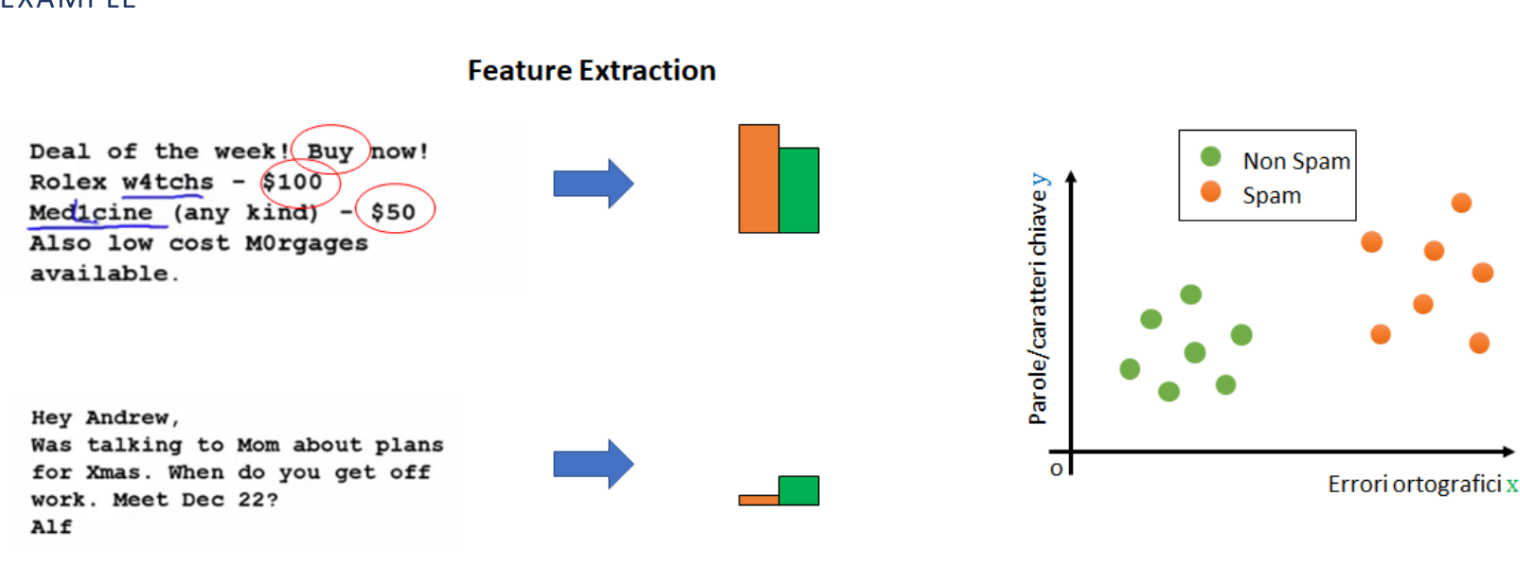
\includegraphics[width=\textwidth]{images/featureExtraction.png}
    \caption{Estrazione delle feature: le e-mail vengono trasformate in vettori 2D, dove $x = \text{errori ortografici e } y = \text{pattern ripetibili}$, e proiettate nello spazio delle feature, , dove la separazione tra spam (arancione) e non spam (verde) risulta evidente.}
    \label{fig:featureExtraction}
\end{figure}

\section{Tipologie di Task}

Le attività possono essere di diversi tipi. Di seguito, discuteremo due compiti principali:

\begin{itemize}
\item \textbf{Classificazione}
\item \textbf{Regressione}
\end{itemize}

Assumeremo che ogni algoritmo di apprendimento automatico prenda come input esempi che sono già stati rappresentati con una funzione di rappresentazione adeguata.

\subsection{Classificazione}

In questo tipo di attività, alla macchina viene chiesto di specificare a quale di un insieme predefinito di categorie $K$ appartiene l'input.

\noindent
Esempi di questo compito sono:

\begin{itemize}
\item Classificare i post di Facebook come riguardanti la politica o qualcos'altro (classificazione politica vs non politica).
\item Rilevamento delle e-mail di spam (classificazione dello spam vs legittima delle e-mail).
\item Riconoscimento dell'oggetto raffigurato in un'immagine tra 1000 oggetti diversi (riconoscimento dell'oggetto).
\end{itemize}

\noindent
L'algoritmo di apprendimento è solitamente fornito con un insieme di esempi:

$$ \{x^{(1)}, x^{(2)}, ..., x^{(n)}\} \text{ dove: } x^{(j)} \in \mathbb{R}^{N} \forall j$$

\noindent
e un insieme di etichette corrispondenti

$$ \{y^{(1)}, y^{(2)}, ..., y^{(n)}\} \text{ dove: } y^{(j)} \in \{1,..,k\}\forall j$$

\noindent
che specificano a quale delle categorie K appartiene ogni esempio.

Ad esempio, se $y^{(j)} = 3$, allora $x^{(j)} $ appartiene alla classe "3".

Nel caso della classificazione binaria (ad esempio, spam vs non spam), $y^{(j)} \in \{0,1\} $. Per risolvere questo compito, l'algoritmo di apprendimento automatico assume la forma di una funzione:

$$ h_\theta: \mathbb{R}^{N} \rightarrow \{1, ... ,K\} $$

\noindent
tale che:

$$y^{(j)} = h_\theta(x^{(j)})$$

\noindent
Esempio:

\begin{itemize}
    \item \textbf{Classification Task:} data un'e-mail, classificarla come spam o non spam.
    \item \textbf{Input:} esempi n-dimensionali $ x = (x_1, x_2, ..., x_n)$ contenenti le caratteristiche dell'email, come il numero di errori ortografici e l'occorrenza di parole specifiche.
    \item \textbf{Output:} etichette $y \in \{0,1\}$ che indicano se l'e-mail è legittima o spam.
\end{itemize}

Alcuni algoritmi di classificazione \textbf{non prevedono un output discreto}, ma un vettore di \textbf{probabilità}, contenente la probabilità relativa a ciascuna delle etichette possibili. In questo caso, puntiamo ad avere la probabilità massima nello slot del vettore relativo all'etichetta vera. 

\subsection{Regressione}

In questo tipo di compito, al programma del computer viene chiesto di \textbf{prevedere un valore numerico dato un input}, tipo:
\begin{itemize}
    \item Prevedere il prezzo delle case date alcune caratteristiche come la città, l'età, la zona, ecc.
    \item Prevedere il valore futuro delle azioni di una società dai valori di altre società o da altre statistiche sul mercato (previsione del mercato azionario).
    \item Conta il numero di auto presenti in un'immagine.
\end{itemize}

\noindent
Analogamente alla classificazione, l'algoritmo viene fornito con esempi di training $x \in \mathbb{R}^{N}$ e con gli output desiderati $y \in \mathbb{R}$. L'algoritmo di apprendimento automatico assume la forma di una funzione $ h_\theta: \mathbb{R}^{N} \rightarrow \mathbb{R}$ tale che $y^{(j)} = h_\theta(x^{(j)})$.

\noindent
Esempio:

\begin{itemize}
    \item \textbf{Regression task:} Predire il prezzo di una casa in base ai suoi metri quadrati.
    \item \textbf{Input:} Dimensione della casa $x$ (valore scalare)
    \item \textbf{Output:} Prezzo $y$.
\end{itemize}

\noindent
Sono algoritmi ottimi per trovare relazioni tra i dati ed effettuare predizioni.

\begin{figure}[htp]
    \centering
    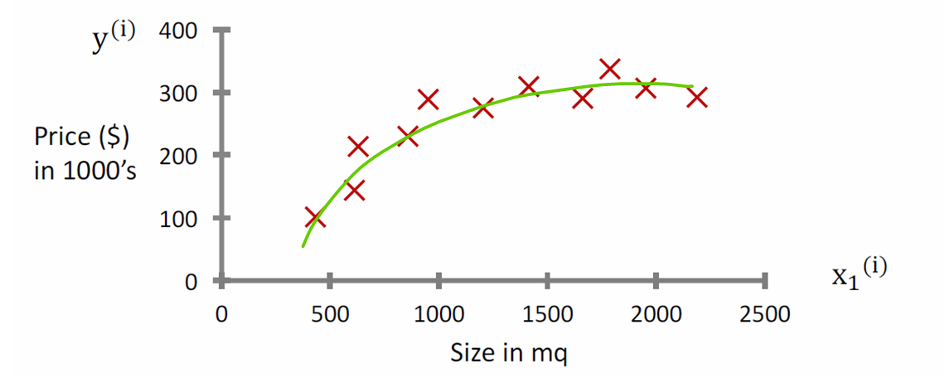
\includegraphics[width=\textwidth]{images/regression.png}
    \caption{Relazione tra dimensione dell’immobile $(x_11^{(i)}$, in mq) e prezzo $(y^{(i)}$, in migliaia di \$): i punti rossi sono i dati osservati, la linea blu rappresenta un modello di regressione lineare che non approssima bene l’andamento non lineare.}
    \label{fig:regressione}
\end{figure}

\newpage
\section{Supervised Learning e Unsupervised Learning}

Gli approcci di Machine Learning possono essere approssimativamente divisi in \textbf{supervised} e \textbf{unsupervised learning}.

\paragraph{Supervised Learning:} L'algoritmo viene addestrato su un insieme di esempi di input e \textbf{output desiderati}. L'obiettivo è allenare un modello a mappare gli input agli output corretti. Il punto chiave qui è il conoscere gli output desiderati: i dati del nostro dataset dovranno quindi essere preventivamente \textbf{etichettati}.

\paragraph{Unsupervised Learning:} L'algoritmo viene addestrato solo su esempi di input, senza output desiderati. L'obiettivo è trovate struttura, pattern e associazioni nei dati, spesso molto eterogenei.

$$ 
\{x^{(1)}, x^{(2)}, ..., x^{(n)}\} \qquad \text{ dove: } x^{(j)} \in \mathbb{R}^{N} \forall j
$$

Questi tipi di compiti mirano generalmente a \textbf{modellare la struttura dei dati}. Un esempio di unsupervised learning è il \textbf{clustering}, in cui non viene fornita alcuna informazione aggiuntiva oltre agli esempi.

Gli approcci supervised sono generalmente più facili da gestire, ma richiedono la presenza di \textbf{labels}. Ottenere labels è spesso un problema costoso in termini di tempo, poiché richiede che le persone annotino manualmente i dati. Ad esempio, se dobbiamo costruire un spam-detector utilizzando un approccio supervised, è necessario che qualcuno etichetti manualmente diverse email come ‘spam’ o ‘non-spam’.

\newpage

\section{Reinforcement Learning}

Alcuni autori fanno riferimento anche a una terza classe di algoritmi di Machine Learning: il \textbf{Reinforcement Learning}.

Il Reinforcement Learning mira a \textbf{scoprire la soluzione a un problema} attraverso il metodo \emph{trial and error}, piuttosto che tramite istruzioni esplicite su come risolvere il compito. Questo avviene permettendo all'algoritmo di \textbf{interagire con un environment} e ricevere \textbf{positive rewards} quando compie azioni che portano a un buon risultato (rispetto al problema da risolvere) e \textbf{negative rewards} quando compie azioni che portano a un risultato negativo.

L'obiettivo degli algoritmi di Reinforcement Learning è apprendere una policy $\pi$, che possa essere utilizzata per \textbf{determinare quale azione a intraprendere} quando si acquisisce un'\textbf{osservazione} del mondo $o$. Questo processo \textbf{ricorda il modo naturale in cui gli animali imparano a risolvere problemi}. Ad esempio, si può pensare a un topo che deve trovare l'uscita da un labirinto (immagine \ref{fig:reinforcementLearning}).

\begin{figure}[htp]
    \centering
    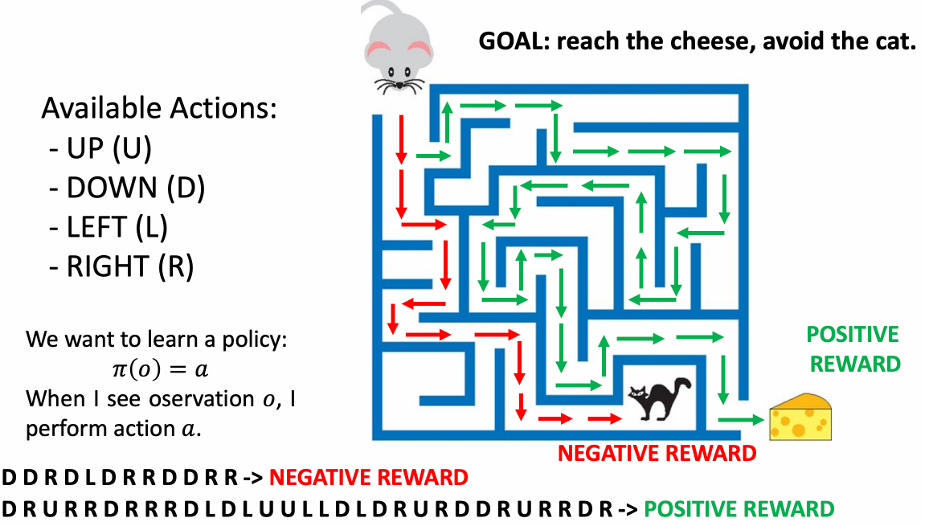
\includegraphics[width=\textwidth]{images/reinforcementLearning.png}
    \caption{Reinforcement Learning nel labirinto: l’agente sceglie tra azioni U/D/L/R e apprende una policy \(\pi(o)=a\) che massimizza la ricompensa, raggiungendo il formaggio (positiva) ed evitando il gatto (negativa).}
\label{fig:reinforcementLearning}
\end{figure}

\section{Misura di Performance (P)}

Per valutare le capacità di un algoritmo di Machine Learning nel risolvere un determinato compito, è necessaria una misura quantitativa delle sue prestazioni. Solitamente, questa \textbf{performance measure} \( P \) è \textbf{specifica per il task} \( T \) che il sistema sta eseguendo.

Per compiti come la classification, spesso si misura la performance utilizzando l'\textbf{accuracy}, ovvero la percentuale di esempi classificati correttamente dal modello. Nel caso della regression, invece, si possono usare altre metriche come il mean squared error.

\noindent
Le misure di performance sono utilizzate per due motivi principali:

\begin{itemize}
\item Capire quando un algoritmo di Machine Learning sta migliorando in un determinato compito.
\item Valutare la performance dell'algoritmo una volta finalizzato.
\end{itemize}

\noindent
Una performance measure può anche essere vista in termini di error. Ad esempio, l'\textbf{accuracy} corrisponde a un error rate (la percentuale di esempi classificati in modo errato), calcolato come \( 1 - accuracy \).

\subsection{Esempio}

Un spam detector analizza cinque email. Le prime tre sono spam, le ultime due non lo sono. L'algoritmo classifica come spam le prime due email e come non spam le ultime tre. In questo caso, la prima e le ultime due classificazioni sono corrette, mentre la terza è errata. La accuracy si calcola come la percentuale di esempi classificati correttamente:

$$
\frac{4}{5} = 0.8 \quad \text{ovvero} \quad 80\%
$$

\section{Experience (E)}

Un algoritmo di Machine Learning apprende dall'\textbf{experience} per migliorare una performance measure su un determinato task.

\noindent
L'\textbf{experience} è costituita da una raccolta di esempi

\[
 x^{(i)}
\]

\noindent
(noti anche come data points, poiché possono essere mappati in uno spazio multi-dimensionale tramite una funzione di rappresentazione), eventualmente accompagnati dalle relative labels 

\[ y^{(i)} \]

\noindent
(a seconda del task considerato).

\noindent
Esistono due principali tipi di algoritmi di Machine Learning:

\begin{itemize}
\item Supervised approaches (quando abbiamo le paired labels, ad esempio nella classification e nella \textbf{regression}).
\item Unsupervised approaches (quando non abbiamo paired labels, come nel \textbf{clustering}).
\end{itemize}

\noindent
L'\textbf{experience} assume forme diverse a seconda del tipo di approccio di Machine Learning utilizzato.

\section{Dataset (D)}

Le performance measures vengono generalmente calcolate rispetto a un insieme di esempi, piuttosto che su singoli esempi. Un insieme di esempi (eventualmente con labels) è chiamato \textbf{dataset}. I datasets sono generalmente omogenei, nel senso che i dati contenuti al loro interno hanno un formato simile. Ad esempio:

\begin{itemize}
    \item Nel Fisher’s Iris dataset, tutti gli esempi hanno 4 features e una label corrispondente a una delle tre classi.
    \item In un dataset di immagini di food, ogni immagine è associata a una class che indica il piatto specifico.
\end{itemize}

\section{Design Matrix}

Un modo comune per rappresentare un dataset è utilizzare una design matrix. Poiché ogni esempio è una collezione di $n$ features, un dataset di $m$ elementi può essere rappresentato tramite una matrice

$$
X \in \mathbb{R}^{m \times n}, \ m, n \in \mathbb{N}
$$

\noindent
di dimensione $m \times n$.

\begin{itemize}
    \item Ogni riga della design matrix rappresenta un esempio.
    \item Ogni colonna rappresenta una delle features.
\end{itemize}

\noindent
Nel caso del supervised learning, si considera spesso anche un'altra matrice

$$ Y \in \mathbb{A}^{m \times k}, k \in \mathbb{N}$$

\noindent
dove \( k \) è la dimensionalità degli output desiderati.

\noindent
Ad esempio, nel caso della classification,

\[ \mathbb{A} = \{1, \ldots, M\} \]

\noindent
dove \( M \) è il numero di classi e k è spesso uguale a 1.

\begin{figure}[htbp]
    \centering
    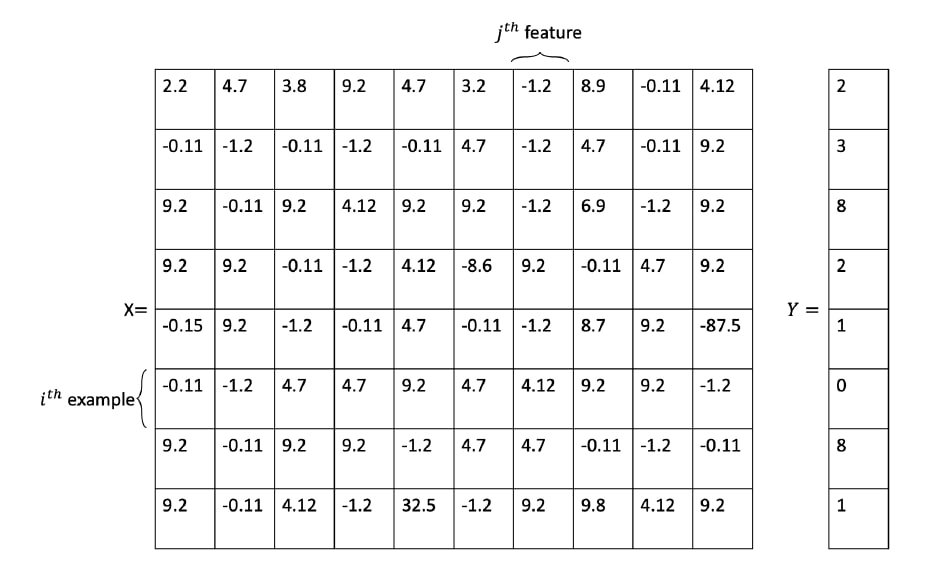
\includegraphics[width=\textwidth]{images/designMatrix.jpg}
    \caption{Design Matrix: rappresentazione di un dataset con m esempi e n features. Ogni riga corrisponde a un esempio, ogni colonna a una feature.}
    \label{fig:designMatrix}
\end{figure}

\subsection{Esempio}

Supponiamo di avere un dataset composto da 1000 email, alcune classificate come spam e altre come not spam. Assumiamo che ogni email sia rappresentata da due features, come discusso nei precedenti esempi.

\noindent
La design matrix che rappresenta il dataset è una matrice

$$ X \in \mathbb{R}^{1000 \times 2} $$

\begin{itemize}
\item Ogni elemento della matrice rappresenta una delle features di un esempio nel dataset.
\item Ad esempio, $ {X}_{i,1} $ indica il numero di \textbf{errori} ortografici nell’$i$-\textbf{esima email}, mentre $ {X}_{j,2} $ rappresenta il numero di \textbf{occorrenze} di parole chiave nell’$j$-\textbf{esima email}, e così via.
\end{itemize}

\noindent
Le labels sono contenute in un vettore

$$ Y \in \{0,1\}^{1000} $$
dove $ Y_i $ rappresenta la label associata all’$i$-\textbf{esimo esempio} (ad esempio, 0 = not spam, \textbf{1 = spam}).

\section{Learning}

Un algoritmo di Machine Learning \textbf{utilizza un dataset di esempi} per \textbf{migliorare la sua performance} in un determinato \textbf{task}. Il processo di miglioramento della performance dell'algoritmo è chiamato \textbf{learning} o \textbf{training}.

\subsection{In cosa consiste il training?}

\begin{itemize}
\item Un algoritmo di Machine Learning ha alcuni parametri chiamati parameters, che possono essere regolati per modificarne il comportamento. Questi parametri sono legati a un model (una funzione matematica) utilizzata per risolvere il task.
\item Un algoritmo chiamato training procedure utilizza gli esempi forniti per trovare i valori ottimali per questi parameters.
\item Alcuni parametri non possono essere regolati automaticamente dal training. Questi sono detti hyperparameters e devono essere ottimizzati al di fuori della training procedure, spesso attraverso un metodo trial and error.
\end{itemize}

\subsection{Esempio}

Consideriamo un semplice spam detector che classifica le email come spam o non-spam in base al numero di errori ortografici. 

\noindent
L'algoritmo può essere scritto come segue:


\begin{lstlisting}[style=py,caption={Soglia sul numero di errori ortografici, chiaramente un approccio naive},label={lst:spam-threshold}]
def classify(x):
    if x > a:
        return 1  # Spam
    else:
        return 0  # Non-spam
\end{lstlisting}

\noindent
L'algoritmo dipende da un singolo parametro $a$. La domanda è: quale valore dovremmo assegnare ad $a$? La \emph{training procedure} permette di trovare un valore ottimo presumibilmente adatto per $a$.
\noindent
Una semplice training procedure consisterebbe nel provare diversi valori per $a$ e registrare le performance dell'algoritmo per ciascun valore di $a$. Alla fine, possiamo scegliere il valore di $a$ che massimizza la performance measure P.

\section{Il paradigma Training/Testing}
	Ciascun algoritmo di Machine Learning presenta al suo interno dei parametri. Una scelta opportuna dei parametri, dovrebbe garantire il funzionamento del modello. La procedura generale, per la scelta e la verifica dei parametri dell'algoritmo, è suddivisa in due parti:

\begin{enumerate}
	\item \textbf{Training dell'algoritmo}.\\
	Effettuato usando i dati dell'omonimo \textbf{training set}, consiste nella scelta dei parametri del modello, vedendo ogni volta i valori della \textit{loss function}, o funzione di costo, che offre un'indice dell'errore da parte del modello, permettendo di capire se i parametri vanno modificati, e di quanto.
	\item \textbf{Testing dell'algoritmo - Inferenza.}\\
	Passiamo ora ai dati di testing, usati per verificare se i parametri scelti sul dataset di training, sono opportuni su dati mai visti prima. Andremo a valutare quindi il nostro modello, secondo quelle che chiamiamo \textbf{misure di valutazione}.
\end{enumerate}

\newpage

\section{Sui dati}

\subsection{Testing - Training}
Come accennato in precedenza, distinguiamo due insiemi di dati: i \textbf{dati di training} e i \textbf{dati di testing}. È importante che i dati usati in fase di training, e i dati usati in fase di inferenza, siano \textbf{totalmente disgiunti}. 
$$
\text{Training }\cap \text{Testing} = \varnothing
$$

Tuttavia, entrambi i set di dati appartengono in origine all'insieme $X$. La suddivisione dei dati in training e testing sarà effettuata randomicamente, in modo da evitare bias di qualsiasi tipo. Dobbiamo inoltre assicurarci che il numero di dati, per ogni etichetta, sia uguale. Prendere l'80\% di un dataset in fase di testing, con due classi (Cane, non-cane), significa prendere l'80\% di ciascuna delle due classi. L'obiettivo è \textbf{evitare favoritismi} durante la classificazione. Parleremo più avanti di tecniche che stabiliscono come effettuare la suddivisione tra training e testing, sfruttando al meglio i propri dati, come la $k$-fold cross-validation.


\subsection{Normalizzazione}
I nostri dati $x \in \mathbb{R}^d$ possono avere valori appartenenti a range molto ampi, con range diversi per ciascuna di queste features. Per creare spazi in cui le features hanno più o meno la stessa dimensione, si usano delle strategie di normalizzazione, come: 

\begin{itemize}
	\item Normalizzazione in $[0,1]$:\\
	Per ogni $j$-esima feature, dobbiamo andare a stabilire il minimo e il massimo del dataset. Dato un dataset di dimensione $m$:
	
	$$
	x_j^{\min } = \min\{x_j^{(i)} | i = 1, 2, \dots, m\}, \qquad 
	x_j^{\max} = \max\{x_j^{(i)} | i = 1, 2, \dots, m\}
	$$
	
	Possiamo quindi normalizzare secondo la seguente formula:
	$$
	\hat{x}_j = \frac{x_j - x_j^{\min}}{x_j^{\max} - x_j^{\min}}
	$$
	
	Ogni dato sarà $\hat{x}_j \in [0,1]$.
	
	\item Normalizzazione in $[-1,1]$:\\
	$$
	\frac{x_j - \mu_j}{\sigma_j}
	$$
	
	con $\sigma_j$ varianza. Il risultato è un centramento a $(0,0)$ dei nostri dati. L'origine coinciderà con la nostra media. Ogni dato sarà $\hat{x}_j \in [-1,1]$.
	
\end{itemize}

Bisognerà conservare rispettivamente $x_j^{\min }, x_j^{\max }$ o $\mu_j, \sigma_j$, per permettere la normalizzazione del testing set, in quanto la normalizzazione è fatta in fase di training.

\section{Iperparametri}
Sono dei parametri che stabiliscono aspetti del nostro modello, e che non sono calcolati in fase di training.
In fase di training, questi vengono fissati, e \textbf{non influiscono sul training}. Nonostante ciò, gli iperparametri avranno un effetto sulla nostra loss-function. Bisognerà variare gli iperparametri usando un \textbf{validation set}, un terzo set di dati sempre ottenuto dal dataset $X$.

\subsection{k-fold Cross Validation}
È una strategia che permette di ottenere ottimi risultati anche con dataset più piccoli.

Dividiamo in due parti il nostro dataset $X$, ottenendo l'insieme di training e l'insieme di testing. Dividiamo nuovamente l'insieme di \textbf{training }in $k$ parti. Supporremo $k=3$. Utilizzeremo un $\frac{1}{k}$ per la validazione e le $\frac{k-1}{k}$ rimanenti come training. In questo caso, $1/3$ e $2/3$. Effettueremo tre volte training e validazione, variando ogni volta il subset usato per la validazione e quelli usati per il testing. Da ciascuno dei processi di training, emergerà un valore della loss function: sceglierò gli iperparametri associati a valori della loss function più bassi.

\begin{figure}[htbp]
	\centering
	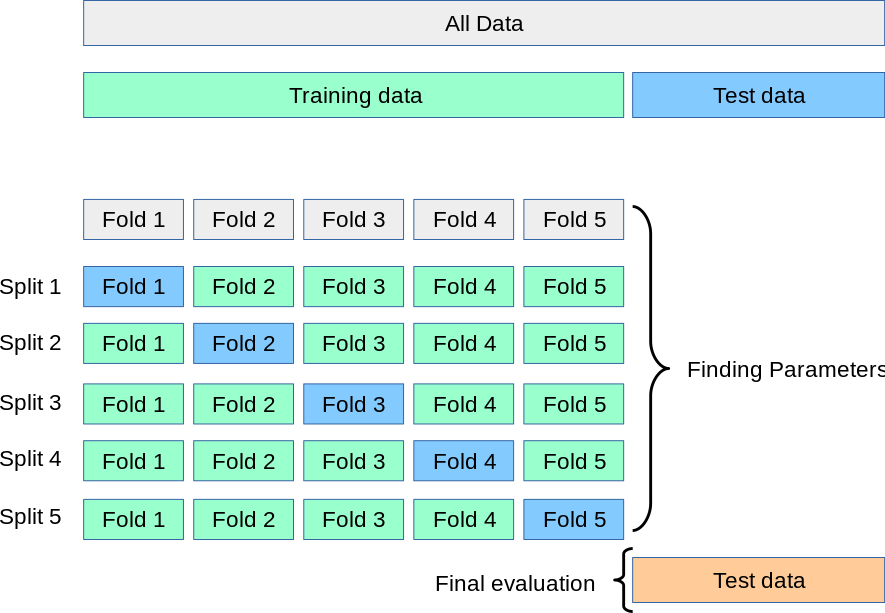
\includegraphics[width=\textwidth]{images/cross_validation.png}
	\caption{Procedura di cross-validation con $k=5$.}
	\label{fig:featureExtraction}
\end{figure}

\newpage

\section{Overfitting e underfitting}
Sono tra i problemi più grandi che possono emergere con i propri algoritmi di machine learning, e riguardano spesso la \textbf{scelta del modello}. 

\begin{itemize}
	\item \textbf{Overfitting}.\\
	Generalmente si parla di overfitting, quando il modello è così complesso da offrire performance ottime in fase di training (impara facilmente e bene), ma fortemente \textbf{peggiori in fase di testing}: il modello è così complesso da imparare troppo bene i dati su cui ha appreso, ma da pessime performance sui dati inediti. 
	\item \textbf{Underfitting.}\\
	Caratterizzato da \textbf{pessime performance in fase di training}, troppe poche variabili, modello troppo semplice. L'apprendimento non è tale da permettere al modello di conoscere il proprio dataset. Il modello non impara!
\end{itemize}

\begin{figure}[htbp]
	\centering
	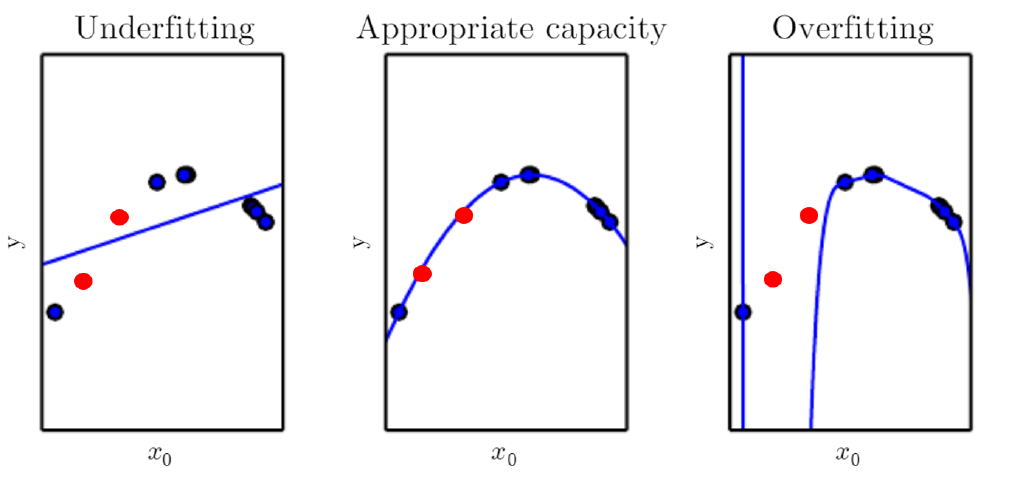
\includegraphics[width=\textwidth]{images/underoverfitting}
	\caption{In blu i dati di training, in rosso quelli di testing. Nel caso dell'underfitting, vediamo una funzione troppo semplice (una funzione lineare) per approssimare una funzione più complessa. Nel caso dell'overfitting, il modello da output assurdi.}
	\label{fig:underoverfitting}
\end{figure}

Bisogna quindi trovare lo \textit{sweetspot}, il compromesso, tra i modelli più complessi, e quelli più semplici. Il numero di parametri è un fattore da tenere sempre in considerazione. 

\subsection{Bias e Variance}

Osservando i risultati dei nostri modelli, sarà possibile individuare facilmente due tipologie di errori:
\begin{itemize}
	\item \textbf{Bias error}.\\
	Modelli troppo semplici non si avvicinano abbastanza ai risultati attesi. Usare modelli con alto bias causa underfitting.
	\item \textbf{Variance error}.\\
	Modelli troppo complessi e ad alta varianza nei risultati, presentano overfitting. L'alta varianza ci fa intuire che il rumore nei nostri dati, influenza esageratamente i risultati.
\end{itemize}





\backmatter
% (eventuali appendici)
% \appendix
% \include{appendici}

% (eventuale bibliografia)
% \bibliographystyle{plain}
% \bibliography{bibliografia}

\end{document}